\documentclass{article}
\usepackage{fullpage}
\usepackage{mathptmx}
\usepackage{graphicx}
\usepackage{amsmath}
\usepackage[aux]{rerunfilecheck}

\newcommand{\ds}{\displaystyle}

% Macros for MATH 110 course dates

\newcommand{\commonTheme}{metropolis}
\newcommand{\commonColorTheme}{metropolis}

\newcommand{\commonAuthor}{Edward Doolittle}
\newcommand{\commonInstitute}{Department of Indigenous Knowledge and
  Science \\ First Nations University of Canada}
\newcommand{\commonCourse}{MATH 110 Calculus I}
\newcommand{\commonTerm}{202510}
\newcommand{\commonDate}{January 6, 2025}

% Review Material

% Lab 0
\newcommand{\commonEventNegativeOne}{LabNegativeOne}
\newcommand{\commonDateLabNegativeOne}{Monday, January 6, 2025}
\newcommand{\commonTitleLabNegativeOne}{MATH 110 Lab 0}
\newcommand{\commonSubtitleLabNegativeOne}{No Lab; Course Opens}

% Section 001
\newcommand{\commonEventZeroZeroOne}{ZeroZeroOne}
\newcommand{\commonDateZeroZeroOne}{Tuesday, January 7, 2025}
\newcommand{\commonTitleZeroZeroOne}{MATH 110 Review 0.1}
\newcommand{\commonSubtitleZeroZeroOne}{Review of Algebra}
\newcommand{\commonPSTitleZeroZeroOne}{MATH 110 Review Problem Set 0.1}

% Section 00A
\newcommand{\commonEventZeroZeroA}{ZeroZeroA}
\newcommand{\commonDateZeroZeroA}{Tuesday, January 7, 2025}
\newcommand{\commonTitleZeroZeroA}{MATH 110 Review 0.A}
\newcommand{\commonSubtitleZeroZeroA}{Review of Inequalities and
  Absolute Values}
\newcommand{\commonPSTitleZeroZeroA}{MATH 110 Review Problem Set 0.A}

% Section 00B
\newcommand{\commonEventZeroZeroB}{ZeroZeroB}
\newcommand{\commonDateZeroZeroB}{Tuesday, January 7, 2025}
\newcommand{\commonTitleZeroZeroB}{MATH 110 Review 0.B}
\newcommand{\commonSubtitleZeroZeroB}{Review of Coordinate Geometry
  and Lines}
\newcommand{\commonPSTitleZeroZeroB}{MATH 110 Review Problem Set 0.B}

% Section 00C
\newcommand{\commonEventZeroZeroC}{ZeroZeroC}
\newcommand{\commonDateZeroZeroC}{Thursday, January 9, 2025}
\newcommand{\commonTitleZeroZeroC}{MATH 110 Review 0.C}
\newcommand{\commonSubtitleZeroZeroC}{Review of Graphs of Second
  Degree Equations}
\newcommand{\commonPSTitleZeroZeroC}{MATH 110 Review Problem Set 0.C}

% Section 00D
\newcommand{\commonEventZeroZeroD}{ZeroZeroD}
\newcommand{\commonDateZeroZeroD}{Thursday, January 9, 2025}
\newcommand{\commonTitleZeroZeroD}{MATH 110 Review 0.D}
\newcommand{\commonSubtitleZeroZeroD}{Review of Trigonometry}
\newcommand{\commonPSTitleZeroZeroD}{MATH 110 Review Problem Set 0.D}

% Section 011
\newcommand{\commonEventZeroOneOne}{ZeroOneOne}
\newcommand{\commonDateZeroOneOne}{Thursday, January 9, 2025}
\newcommand{\commonTitleZeroOneOne}{MATH 110 Review 1.1}
\newcommand{\commonSubtitleZeroOneOne}{Review of Functions}
\newcommand{\commonPSTitleZeroOneOne}{MATH 110 Review Problem Set 1.1}


% Main Course

% Lab 1
\newcommand{\commonEventZero}{LabZero}
\newcommand{\commonDateLabZero}{Monday, January 13, 2025}
\newcommand{\commonTitleLabZero}{MATH 110 Lab 1}
\newcommand{\commonSubtitleLabZero}{Quiz 0: STACK, Onboarding}

% Section 1.4
\newcommand{\commonEventOne}{ZeroOneFour}
\newcommand{\commonDateZeroOneFour}{Tuesday, January 14, 2025}
\newcommand{\commonTitleZeroOneFour}{MATH 110 Lecture 1.4}
\newcommand{\commonSubtitleZeroOneFour}{The Tangent and Velocity Problems}
\newcommand{\commonPSTitleZeroOneFour}{MATH 110 Problem Set 1.4}

% Section 1.5
\newcommand{\commonEventTwo}{ZeroOneFive}
\newcommand{\commonDateZeroOneFive}{Thursday, January 16, 2025}
\newcommand{\commonTitleZeroOneFive}{MATH 110 Lecture 1.5}
\newcommand{\commonSubtitleZeroOneFive}{The Limit of a Function}
\newcommand{\commonPSTitleZeroOneFive}{MATH 110 Problem Set 1.5}

% Lab 2
\newcommand{\commonEventThree}{LabOne}
\newcommand{\commonDateLabOne}{Monday, January 20, 2025}
\newcommand{\commonTitleLabOne}{MATH 110 Lab 2}
\newcommand{\commonSubtitleLabOne}{Quiz 1: Review}

% Section 1.6
\newcommand{\commonEventFour}{ZeroOneSix}
\newcommand{\commonDateZeroOneSix}{Tuesday, January 21, 2025}
\newcommand{\commonTitleZeroOneSix}{MATH 110 Lecture 1.6}
\newcommand{\commonSubtitleZeroOneSix}{Calculating Limits Using the Limit Laws}
\newcommand{\commonPSTitleZeroOneSix}{MATH 110 Problem Set 1.6}

% Section 1.7
\newcommand{\commonEventFive}{ZeroOneSeven}
\newcommand{\commonDateZeroOneSeven}{(Not covered)}
\newcommand{\commonTitleZeroOneSeven}{MATH 110 Lecture 1.7}
\newcommand{\commonSubtitleZeroOneSeven}{The Precise Definition of a Limit}
\newcommand{\commonPSTitleZeroOneSeven}{MATH 110 Problem Set 1.7}

% Section 1.8
\newcommand{\commonEventSix}{ZeroOneEight}
\newcommand{\commonDateZeroOneEight}{Thursday, January 23, 2025}
\newcommand{\commonTitleZeroOneEight}{MATH 110 Lecture 1.8}
\newcommand{\commonSubtitleZeroOneEight}{Continuity}
\newcommand{\commonPSTitleZeroOneEight}{MATH 110 Problem Set 1.8}

% Lab 3
\newcommand{\commonEventSeven}{LabTwo}
\newcommand{\commonDateLabTwo}{Monday, January 27, 2025}
\newcommand{\commonTitleLabTwo}{MATH 110 Lab 3}
\newcommand{\commonSubtitleLabTwo}{Quiz 2: Sections 1.4, 1.5}

% Section 2.1
\newcommand{\commonEventEight}{ZeroTwoOne}
\newcommand{\commonDateZeroTwoOne}{Tuesday, January 28, 2025}
\newcommand{\commonTitleZeroTwoOne}{MATH 110 Lecture 2.1}
\newcommand{\commonSubtitleZeroTwoOne}{Derivatives and Rates of Change}
\newcommand{\commonPSTitleZeroTwoOne}{MATH 110 Problem Set 2.1}

% Section 2.2
\newcommand{\commonEventNine}{ZeroTwoTwo}
\newcommand{\commonDateZeroTwoTwo}{Thursday, January 30, 2025}
\newcommand{\commonTitleZeroTwoTwo}{MATH 110 Lecture 2.2}
\newcommand{\commonSubtitleZeroTwoTwo}{The Derivative as a Function}
\newcommand{\commonPSTitleZeroTwoTwo}{MATH 110 Problem Set 2.2}

% Lab 4
\newcommand{\commonEventTen}{LabThree}
\newcommand{\commonDateMTOne}{Monday, February 3, 2025} 
\newcommand{\commonDateLabThree}{Monday, February 3, 2025}
\newcommand{\commonTitleLabThree}{MATH 110 Lab 4}
\newcommand{\commonSubtitleLabThree}{Midterm: Review, Chapter 1}

% Section 2.3
\newcommand{\commonEventEleven}{ZeroTwoThree}
\newcommand{\commonDateZeroTwoThree}{Tuesday, February 4, 2025}
\newcommand{\commonTitleZeroTwoThree}{MATH 110 Lecture 2.3}
\newcommand{\commonSubtitleZeroTwoThree}{Differentiation Formulas}
\newcommand{\commonPSTitleZeroTwoThree}{MATH 110 Problem Set 2.3}

% Section 2.4
\newcommand{\commonEventTwelve}{ZeroTwoFour}
\newcommand{\commonDateZeroTwoFour}{Thursday, February 6, 2025}
\newcommand{\commonTitleZeroTwoFour}{MATH 110 Lecture 2.4}
\newcommand{\commonSubtitleZeroTwoFour}{Derivatives of Trigonometric Functions}
\newcommand{\commonPSTitleZeroTwoFour}{MATH 110 Problem Set 2.4}

% Lab 5
\newcommand{\commonEventThirteen}{LabFour}
\newcommand{\commonDateLabFour}{Monday, February 10, 2025}
\newcommand{\commonTitleLabFour}{MATH 110 Lab 5}
\newcommand{\commonSubtitleLabFour}{Quiz 3: Sections 2.1, 2.2}

% Section 2.5
\newcommand{\commonEventFourteen}{ZeroTwoFive}
\newcommand{\commonDateZeroTwoFive}{Tuesday, February 11, 2025}
\newcommand{\commonTitleZeroTwoFive}{MATH 110 Lecture 2.5}
\newcommand{\commonSubtitleZeroTwoFive}{The Chain Rule}
\newcommand{\commonPSTitleZeroTwoFive}{MATH 110 Problem Set 2.5}

% Section 2.6
\newcommand{\commonEventFifteen}{ZeroTwoSix}
\newcommand{\commonDateZeroTwoSix}{Thursday, February 13, 2025}
\newcommand{\commonTitleZeroTwoSix}{MATH 110 Lecture 2.6}
\newcommand{\commonSubtitleZeroTwoSix}{Implicit Differentiation}
\newcommand{\commonPSTitleZeroTwoSix}{MATH 110 Problem Set 2.6}

% Lab 6
\newcommand{\commonEventSixteen}{LabFive}
\newcommand{\commonDateLabFive}{Monday, February 24, 2025}
\newcommand{\commonTitleLabFive}{MATH 110 Lab 6}
\newcommand{\commonSubtitleLabFive}{Quiz 4: Sections 2.3, 2.4}

% Section 2.7
\newcommand{\commonEventSeventeen}{ZeroTwoSeven}
\newcommand{\commonDateZeroTwoSeven}{Tuesday, February 25, 2025}
\newcommand{\commonTitleZeroTwoSeven}{MATH 110 Lecture 2.7}
\newcommand{\commonSubtitleZeroTwoSeven}{Rates of Change in the
  Natural and Social Sciences}
\newcommand{\commonPSTitleZeroTwoSeven}{MATH 110 Problem Set 2.7}

% Section 2.8
\newcommand{\commonEventEighteen}{ZeroTwoEight}
\newcommand{\commonDateZeroTwoEight}{Thursday, February 27, 2025}
\newcommand{\commonTitleZeroTwoEight}{MATH 110 Lecture 2.8}
\newcommand{\commonSubtitleZeroTwoEight}{Related Rates}
\newcommand{\commonPSTitleZeroTwoEight}{MATH 110 Problem Set 2.8}

% Lab 7
\newcommand{\commonEventNineteen}{LabSix}
\newcommand{\commonDateLabSix}{Monday, March 3, 2025}
\newcommand{\commonTitleLabSix}{MATH 110 Lab 7}
\newcommand{\commonSubtitleLabSix}{Quiz 5: Sections 2.5, 2.6}

% Section 3.1
\newcommand{\commonEventTwenty}{ZeroThreeOne}
\newcommand{\commonDateZeroThreeOne}{Tuesday, March 4, 2025}
\newcommand{\commonTitleZeroThreeOne}{MATH 110 Lecture 3.1}
\newcommand{\commonSubtitleZeroThreeOne}{Maximum and Minimum Values}
\newcommand{\commonPSTitleZeroThreeOne}{MATH 11 Problem Set 3.1}

% Section 3.2
\newcommand{\commonEventTwentyOne}{ZeroThreeTwo}
\newcommand{\commonDateZeroThreeTwo}{Thursday, March 6, 2025}
\newcommand{\commonTitleZeroThreeTwo}{MATH 110 Lecture 3.2}
\newcommand{\commonSubtitleZeroThreeTwo}{The Mean Value Theorem}
\newcommand{\commonPSTitleZeroThreeTwo}{MATH 110 Problem Set 3.2}

% Lab 8
\newcommand{\commonEventTwentyTwo}{LabSeven}
\newcommand{\commonDateMTTwo}{Monday, March 10, 2025}
\newcommand{\commonDateLabSeven}{Monday, March 10, 2025}
\newcommand{\commonTitleLabSeven}{MATH 110 Lab 8}
\newcommand{\commonSubtitleLabSeven}{Midterm: Chapter 2}

% Section 3.3
\newcommand{\commonEventTwentyThree}{ZeroThreeThree}
\newcommand{\commonDateZeroThreeThree}{Tuesday, March 11, 2025}
\newcommand{\commonTitleZeroThreeThree}{MATH 110 Lecture 3.3}
\newcommand{\commonSubtitleZeroThreeThree}{How Derivatives Affect the
  Shape of a Graph}
\newcommand{\commonPSTitleZeroThreeThree}{MATH 110 Problem Set 3.3}

% Section 3.4
\newcommand{\commonEventTwentyFour}{ZeroThreeFour}
\newcommand{\commonDateZeroThreeFour}{Thursday, March 13, 2025}
\newcommand{\commonTitleZeroThreeFour}{MATH 110 Lecture 3.4}
\newcommand{\commonSubtitleZeroThreeFour}{Limits at Infinity;
  Horizontal Asymptotes}
\newcommand{\commonPSTitleZeroThreeFour}{MATH 110 Problem Set 3.4}

% Lab 9
\newcommand{\commonEventTwentyFive}{LabEight}
\newcommand{\commonDateLabEight}{Monday, March 17, 2025}
\newcommand{\commonTitleLabEight}{MATH 110 Lab 9}
\newcommand{\commonSubtitleLabEight}{Quiz 6: Sections 3.1, 3.2}

% Section 3.5
\newcommand{\commonEventTwentySix}{ZeroThreeFive}
\newcommand{\commonDateZeroThreeFive}{Tuesday, March 18, 2025}
\newcommand{\commonTitleZeroThreeFive}{MATH 110 Lecture 3.5}
\newcommand{\commonSubtitleZeroThreeFive}{Summary of Curve Sketching}
\newcommand{\commonPSTitleZeroThreeFive}{MATH 110 Problem Set 3.5}

% Section 3.7
\newcommand{\commonEventTwentySeven}{ZeroThreeSeven}
\newcommand{\commonDateZeroThreeSeven}{Thursday, March 20, 2025}
\newcommand{\commonTitleZeroThreeSeven}{MATH 110 Lecture 3.7}
\newcommand{\commonSubtitleZeroThreeSeven}{Optimization Problems}
\newcommand{\commonPSTitleZeroThreeSeven}{MATH 110 Problem Set 3.7}

% Lab 10
\newcommand{\commonEventTwentyEight}{LabNine}
\newcommand{\commonDateLabNine}{Monday, March 24, 2025}
\newcommand{\commonTitleLabNine}{MATH 110 Lab 10}
\newcommand{\commonSubtitleLabNine}{Quiz 7: Sections 3.3, 3.4}

% Section 4.1
\newcommand{\commonEventTwentyNine}{ZeroFourOne}
\newcommand{\commonDateZeroFourOne}{Tuesday, March 25, 2025}
\newcommand{\commonTitleZeroFourOne}{MATH 110 Lecture 4.1}
\newcommand{\commonSubtitleZeroFourOne}{Areas and Distances}
\newcommand{\commonPSTitleZeroFourOne}{MATH 110 Problem Set 4.1}

% Section 4.2
\newcommand{\commonEventThirty}{ZeroFourTwo}
\newcommand{\commonDateZeroFourTwo}{Thursday, March 27, 2025}
\newcommand{\commonTitleZeroFourTwo}{MATH 110 Lecture 4.2}
\newcommand{\commonSubtitleZeroFourTwo}{The Definite Integral}
\newcommand{\commonPSTitleZeroFourTwo}{MATH 110 Problem Set 4.2}

% Lab 11
\newcommand{\commonEventThirtyOne}{LabTen}
\newcommand{\commonDateLabTen}{Monday, March 31, 2025}
\newcommand{\commonTitleLabTen}{MATH 110 Lab 11}
\newcommand{\commonSubtitleLabTen}{Quiz 8: Sections 3.5, 3.7}

% Section 4.3
\newcommand{\commonEventThirtyTwo}{ZeroFourThree}
\newcommand{\commonDateZeroFourThree}{Tuesday, April 1, 2025}
\newcommand{\commonTitleZeroFourThree}{MATH 110 Lecture 4.3}
\newcommand{\commonSubtitleZeroFourThree}{The Fundamental Theorem of Calculus}
\newcommand{\commonPSTitleZeroFourThree}{MATH 110 Problem Set 4.3}

% Section 4.4
\newcommand{\commonEventThirtyThree}{ZeroFourFour}
\newcommand{\commonDateZeroFourFour}{Thursday, April 3, 2025}
\newcommand{\commonTitleZeroFourFour}{MATH 110 Lecture 4.4}
\newcommand{\commonSubtitleZeroFourFour}{Indefinite Integrals and the
  Net Change Theorem}
\newcommand{\commonPSTitleZeroFourFour}{MATH 110 Problem Set 4.4}

% Lab 12
\newcommand{\commonEventThirtyFour}{LabEleven}
\newcommand{\commonDateLabEleven}{Monday, April 7, 2025}
\newcommand{\commonTitleLabEleven}{MATH 110 Lab 12}
\newcommand{\commonSubtitleLabEleven}{Quiz 9: Sections 4.1, 4.2}

% Section 4.5
\newcommand{\commonEventThirtyFive}{ZeroFourFive}
\newcommand{\commonDateZeroFourFive}{Tuesday, April 8, 2025}
\newcommand{\commonTitleZeroFourFive}{MATH 110 Lecture 4.5}
\newcommand{\commonSubtitleZeroFourFive}{The Substitution Rule}
\newcommand{\commonPSTitleZeroFourFive}{MATH 110 Problem Set 4.5}

% Section 5.1
\newcommand{\commonEventThirtySix}{ZeroFiveOne}
\newcommand{\commonDateZeroFiveOne}{Thursday, April 10, 2025}
\newcommand{\commonTitleZeroFiveOne}{MATH 110 Lecture 5.1}
\newcommand{\commonSubtitleZeroFiveOne}{Areas Between Curves}
\newcommand{\commonPSTitleZeroFiveOne}{MATH 110 Problem Set 5.1}

% Lab 13
\newcommand{\commonEventThirtySeven}{LabTwelve}
\newcommand{\commonDateLabTwelve}{Monday, April 14, 2025}
\newcommand{\commonTitleLabTwelve}{MATH 110 Review Lab}
\newcommand{\commonSubtitleLabTwelve}{Bonus Quiz 10: Sections 4.3, 4.4}

% Final Class
\newcommand{\commonEventThirtyEight}{FinalClass}
\newcommand{\commonDateFinalClass}{Tuesday, April 15, 2025}
\newcommand{\commonTitleFinalClass}{MATH 110 Review Class}
\newcommand{\commonSubtitleFinalClass}{Answer Questions, Review for Exam}

% Final Exam
\newcommand{\commonEventThirtyNine}{Final}
\newcommand{\commonDateFinal}{Thursday, April 22, 2025}
\newcommand{\commonTitleFinal}{MATH 110 Final Exam}
\newcommand{\commonSubtitleFinal}{Comprehensive Exam: All Sections}

% Orphaned -- no longer part of the course

% Section 2.9
\newcommand{\commonDateZeroTwoNine}{Not part of the course}
\newcommand{\commonTitleZeroTwoNine}{MATH 110 Lecture 2.9}
\newcommand{\commonSubtitleZeroTwoNine}{Linear Approximations and Differentials}
\newcommand{\commonPSTitleZeroTwoNine}{MATH 110 Problem Set 2.9}


% % Introduction
% \newcommand{\commonEventOneDate}{Wednesday, September 8, 2010}
% \newcommand{\commonEventOneDesc}{Introduction to the Course}
% \newcommand{\commonDateZeroZeroZero}{September 8, 2010}
% \newcommand{\commonTitleZeroZeroZero}{MATH 104 Introduction}
% \newcommand{\commonSubtitleZeroZeroZero}{Outline of the Course}

% % Lecture 1
% \newcommand{\commonEventTwoDate}{Friday, September 10, 2010}
% \newcommand{\commonEventTwoDesc}{Lecture 1: Algebra}
% \newcommand{\commonDateZeroZeroOne}{September 10, 2010}
% \newcommand{\commonTitleZeroZeroOne}{MATH 104 Lecture 1}
% \newcommand{\commonSubtitleZeroZeroOne}{Review of Algebra}
% % associated evaluation ... factor this out?
% \newcommand{\commonPSTitleZeroZeroOne}{MATH 104 Problem Set 1}
% \newcommand{\commonEvalZeroZeroOne}{Quiz 1}
% \newcommand{\commonEvalDateZeroZeroOne}{Wednesday, September 15, 2010}

% % Lecture 2
% \newcommand{\commonEventThreeDate}{Monday, September 13, 2010}
% \newcommand{\commonEventThreeDesc}{Lecture 2: Appendix A}
% \newcommand{\commonDateZeroZeroA}{September 13, 2010}
% \newcommand{\commonTitleZeroZeroA}{MATH 104 Lecture 2}
% \newcommand{\commonSubtitleZeroZeroA}{Appendix A: Numbers, Inequalities, 
%   and Absolute Values}
% % associated evaluation ... factor this out?
% \newcommand{\commonPSTitleZeroZeroA}{MATH 104 Problem Set 2}
% \newcommand{\commonEvalZeroZeroA}{Quiz 2}
% \newcommand{\commonEvalDateZeroZeroA}{Wednesday, September 22, 2010}

% % Review 1
% \newcommand{\commonEventFourDate}{Wednesday, September 15, 2010}
% \newcommand{\commonEventFourDesc}{Review 1: Review Algebra; Quiz 1; Review Appendix A}
% \newcommand{\commonDateRZeroOne}{September 15, 2010}
% \newcommand{\commonTitleRZeroOne}{MATH 104 Review 1}
% \newcommand{\commonSubtitleRZeroOne}{Review of Algebra, Appendix A}

% % Lecture 3
% \newcommand{\commonEventFiveDate}{Friday, September 17, 2010}
% \newcommand{\commonEventFiveDesc}{Lecture 3: Appendix B}
% \newcommand{\commonDateZeroZeroB}{September 17, 2010}
% \newcommand{\commonTitleZeroZeroB}{MATH 104 Lecture 3}
% \newcommand{\commonSubtitleZeroZeroB}{Appendix B: Coordinate Geometry and Lines}
% % associated evaluation ... factor this out?
% \newcommand{\commonPSTitleZeroZeroB}{MATH 104 Problem Set 3}
% \newcommand{\commonEvalZeroZeroB}{Quiz 2}
% \newcommand{\commonEvalDateZeroZeroB}{Wednesday, September 22, 2010}

% % Lecture 4
% \newcommand{\commonEventSixDate}{Monday, Sepbember 20, 2010}
% \newcommand{\commonEventSixDesc}{Lecture 4: Appendix C}
% \newcommand{\commonDateZeroZeroC}{September 20, 2010}
% \newcommand{\commonTitleZeroZeroC}{MATH 104 Lecture 4}
% \newcommand{\commonSubtitleZeroZeroC}{Appendix C: Graphs of Second-Degree Equations}
% % associated evaluation ... factor this out?
% \newcommand{\commonPSTitleZeroZeroC}{MATH 104 Problem Set 4}
% \newcommand{\commonEvalZeroZeroC}{Midterm 0}
% \newcommand{\commonEvalDateZeroZeroC}{Wednesday, September 29, 2010}

% % Review 2
% \newcommand{\commonEventSevenDate}{Wednesday, September 22, 2010}
% \newcommand{\commonEventSevenDesc}{Review 2: Review Appendix B; Quiz 2; Review Appendix C}
% \newcommand{\commonDateRZeroTwo}{September 22, 2010}
% \newcommand{\commonTitleRZeroTwo}{MATH 104 Review 2}
% \newcommand{\commonSubtitleRZeroTwo}{Review of Appendices B and C}

% % Lecture 5
% \newcommand{\commonEventEightDate}{Friday, September 24, 2010}
% \newcommand{\commonEventEightDesc}{Lecture 5: Appendix D}
% \newcommand{\commonDateZeroZeroD}{September 24, 2010}
% \newcommand{\commonTitleZeroZeroD}{MATH 104 Lecture 5}
% \newcommand{\commonSubtitleZeroZeroD}{Appendix D: Trigonometry}
% % associated evaluation ... factor this out?
% \newcommand{\commonPSTitleZeroZeroD}{MATH 104 Problem Set 5}
% \newcommand{\commonEvalZeroZeroD}{Midterm 0}
% \newcommand{\commonEvalDateZeroZeroD}{Wednesday, September 29, 2010}

% % Lecture 6
% \newcommand{\commonEventNineDate}{Monday, September 27, 2010}
% \newcommand{\commonEventNineDesc}{Lecture 6: Section 1.1}
% \newcommand{\commonDateZeroOneOne}{September 27, 2010}
% \newcommand{\commonTitleZeroOneOne}{MATH 104 Lecture 6}
% \newcommand{\commonSubtitleZeroOneOne}{Section 1.1: Four Ways to Represent a Function}
% % associated evaluation ... factor this out?
% \newcommand{\commonPSTitleZeroOneOne}{MATH 104 Problem Set 6}
% \newcommand{\commonEvalZeroOneOne}{Quiz 3}
% \newcommand{\commonEvalDateZeroOneOne}{Wednesday, October 6, 2010}

% % Review 3
% \newcommand{\commonEventTenDate}{Wednesday, September 29, 2010}
% \newcommand{\commonEventTenDesc}{Review 3: Review Appendix D; 
%   Self-Assessment Midterm 0}
% \newcommand{\commonDateRZeroThree}{September 29, 2010}
% \newcommand{\commonTitleRZeroThree}{MATH 104 Review 3}
% \newcommand{\commonSubtitleRZeroThree}{Review of Appendix D}

% % Lecture 7
% \newcommand{\commonEventElevenDate}{Friday, October 1, 2010}
% \newcommand{\commonEventElevenDesc}{Lecture 7: Section 1.2}
% \newcommand{\commonDateZeroOneTwo}{October 1, 2010}
% \newcommand{\commonTitleZeroOneTwo}{MATH 104 Lecture 7}
% \newcommand{\commonSubtitleZeroOneTwo}{Section 1.2: Mathematical Models: A Catalog of Essential Functions}
% % associated evaluation ... factor this out?
% \newcommand{\commonPSTitleZeroOneTwo}{MATH 104 Problem Set 7}
% \newcommand{\commonEvalZeroOneTwo}{Quiz 3}
% \newcommand{\commonEvalDateZeroOneTwo}{Wednesday, October 6, 2010}

% % Lecture 8
% \newcommand{\commonEventTwelveDate}{Monday, October 4, 2010}
% \newcommand{\commonEventTwelveDesc}{Lecture 8: Section 1.3}
% \newcommand{\commonDateZeroOneThree}{October 4, 2010}
% \newcommand{\commonTitleZeroOneThree}{MATH 104 Lecture 8}
% \newcommand{\commonSubtitleZeroOneThree}{Section 1.3: New Functions from Old Functions}
% % associated evaluation ... factor this out?
% \newcommand{\commonPSTitleZeroOneThree}{MATH 104 Problem Set 8}
% \newcommand{\commonEvalZeroOneThree}{Quiz 4}
% \newcommand{\commonEvalDateZeroOneThree}{Wednesday, October 13, 2010}

% % Review 4
% \newcommand{\commonEventThirteenDate}{Wednesday, October 6, 2010}
% \newcommand{\commonEventThirteenDesc}{Review 4: Review 1.1, 1.2; Quiz 3}
% \newcommand{\commonDateROneOne}{October 6, 2010}
% \newcommand{\commonTitleROneOne}{MATH 104 Review 4}
% \newcommand{\commonSubtitleROneOne}{Reveiw of 1.1, 1.2}

% % Lecture 9
% \newcommand{\commonEventFourteenDate}{Friday, October 8, 2010}
% \newcommand{\commonEventFourteenDesc}{Lecture 9: Section 1.4}
% \newcommand{\commonDateZeroOneFour}{October 8, 2010}
% \newcommand{\commonTitleZeroOneFour}{MATH 104 Lecture 9}
% \newcommand{\commonSubtitleZeroOneFour}{Section 1.4: Graphing Calculators and Computers}
% % associated evaluation ... factor this out?
% \newcommand{\commonPSTitleZeroOneFour}{MATH 104 Problem Set 9}
% \newcommand{\commonEvalZeroOneFour}{Quiz 4}
% \newcommand{\commonEvalDateZeroOneFour}{Wednesday, October 13, 2010}

% % Thanksgiving holiday
% \newcommand{\commonEventFifteenDate}{Monday, October 11, 2010}
% \newcommand{\commonEventFifteenDesc}{No class: Thanksgiving holiday}

% % Review 5
% \newcommand{\commonEventSixteenDate}{Wednesday, October 13, 2010}
% \newcommand{\commonEventSixteenDesc}{Review 5: Review 1.3, 1.4; Quiz 4}
% \newcommand{\commonDateROneTwo}{October 13, 2010}
% \newcommand{\commonTitleROneTwo}{MATH 104 Review 5}
% \newcommand{\commonSubtitleOneRTwo}{Review of 1.3, 1.4}

% % Lecture 10
% \newcommand{\commonEventSeventeenDate}{Friday, October 15, 2010}
% \newcommand{\commonEventSeventeenDesc}{Lecture 10: Section 1.5}
% \newcommand{\commonDateZeroOneFive}{October 15, 2010}
% \newcommand{\commonTitleZeroOneFive}{MATH 104 Lecture 10}
% \newcommand{\commonSubtitleZeroOneFive}{Section 1.5: Exponential Functions}
% % associated evaluation ... factor this out?
% \newcommand{\commonPSTitleZeroOneFive}{MATH 104 Problem Set 10}
% \newcommand{\commonEvalZeroOneFive}{Quiz 5}
% \newcommand{\commonEvalDateZeroOneFive}{Wednesday, October 20, 2010}

% % Lecture 11
% \newcommand{\commonEventEighteenDate}{Monday, October 18, 2010}
% \newcommand{\commonEventEighteenDesc}{Lecture 11: Section 1.6}
% \newcommand{\commonDateZeroOneSix}{October 18, 2010}
% \newcommand{\commonTitleZeroOneSix}{MATH 104 Lecture 11}
% \newcommand{\commonSubtitleZeroOneSix}{Section 1.6: Inverse Functions and Logarithms}
% % associated evaluation ... factor this out?
% \newcommand{\commonPSTitleZeroOneSix}{MATH 104 Problem Set 11}
% \newcommand{\commonEvalZeroOneSix}{Midterm 1}
% \newcommand{\commonEvalDateZeroOneSix}{Wednesday, October 27, 2010}

% % Review 6
% \newcommand{\commonEventNineteenDate}{Wednesday, October 20, 2010}
% \newcommand{\commonEventNineteenDesc}{Review 6: Review 1.5; Quiz 5; Review 1.6}
% \newcommand{\commonDateROneThree}{October 20, 2010}
% \newcommand{\commonDateZeroOneR}{October 20, 2010}
% \newcommand{\commonTitleROneThree}{MATH 104 Review 6}
% \newcommand{\commonSubtitleROneThree}{Review of 1.5, 1.6}
% % associated evaluation ... factor this out?
% \newcommand{\commonPSTitleZeroOneR}{MATH 104 Problem Set R1}
% \newcommand{\commonEvalZeroOneR}{Midterm 1}
% \newcommand{\commonEvalDateZeroOneR}{Wednesday, October 27, 2010}

% % Lecture 12
% \newcommand{\commonEventTwentyDate}{Friday, October 22, 2010}
% \newcommand{\commonEventTwentyDesc}{Lecture 12: Section 2.1}
% \newcommand{\commonDateZeroTwoOne}{October 22, 2010}
% \newcommand{\commonTitleZeroTwoOne}{MATH 104 Lecture 12}
% \newcommand{\commonSubtitleZeroTwoOne}{Section 2.1: The Tangent and Velocity Problems}
% % associated evaluation ... factor this out?
% \newcommand{\commonPSTitleZeroTwoOne}{MATH 104 Problem Set 12}
% \newcommand{\commonEvalZeroTwoOne}{Quiz 6}
% \newcommand{\commonEvalDateZeroTwoOne}{Wednesday, November 3, 2010}

% % Lecture 13
% \newcommand{\commonEventTwentyOneDate}{Monday, October 25, 2010}
% \newcommand{\commonEventTwentyOneDesc}{Lecture 13: Section 2.2(a)}
% \newcommand{\commonDateZeroTwoTwoa}{October 25, 2010}
% \newcommand{\commonTitleZeroTwoTwoa}{MATH 104 Lecture 13}
% \newcommand{\commonSubtitleZeroTwoTwoa}{Section 2.2(a): The Limit of a Function I}
% % associated evaluation ... factor this out?
% \newcommand{\commonPSTitleZeroTwoTwoa}{MATH 104 Problem Set 13}
% \newcommand{\commonEvalZeroTwoTwoa}{Quiz 6}
% \newcommand{\commonEvalDateZeroTwoTwoa}{Wednesday, November 3, 2010}

% % Midterm Test 1
% % October 27, 2010
% \newcommand{\commonEventTwentyTwoDate}{Wednesday, October 27, 2010}
% \newcommand{\commonEventTwentyTwoDesc}{Midterm Test 1: Chapter 1}

% % Lecture 14
% \newcommand{\commonEventTwentyThreeDate}{Friday, October 29, 2010}
% \newcommand{\commonEventTwentyThreeDesc}{Lecture 14: Section 2.2(b)}
% \newcommand{\commonDateZeroTwoTwob}{October 29, 2010}
% \newcommand{\commonTitleZeroTwoTwob}{MATH 104 Lecture 14}
% \newcommand{\commonSubtitleZeroTwoTwob}{Section 2.2(b): The Limit of a Function II}
% % associated evaluation ... factor this out?
% \newcommand{\commonPSTitleZeroTwoTwob}{MATH 104 Problem Set 14}
% \newcommand{\commonEvalZeroTwoTwob}{Quiz 6}
% \newcommand{\commonEvalDateZeroTwoTwob}{Wednesday, November 3, 2010}

% % Lecture 15
% \newcommand{\commonEventTwentyFourDate}{Monday, November 1, 2010}
% \newcommand{\commonEventTwentyFourDesc}{Lecture 15: Section 2.3}
% \newcommand{\commonDateZeroTwoThree}{November 1, 2010}
% \newcommand{\commonTitleZeroTwoThree}{MATH 104 Lecture 15}
% \newcommand{\commonSubtitleZeroTwoThree}{Section 2.3: Calculating Limits Using the Limit Laws}
% % associated evaluation ... factor this out?
% \newcommand{\commonPSTitleZeroTwoThree}{MATH 104 Problem Set 15}
% \newcommand{\commonEvalZeroTwoThree}{Quiz 7}
% \newcommand{\commonEvalDateZeroTwoThree}{Wednesday, November 10, 2010}

% % Review 7
% \newcommand{\commonEventTwentyFiveDate}{Wednesday, November 3, 2010}
% \newcommand{\commonEventTwentyFiveDesc}{Review 7: Review 2.1, 2.2; Quiz 6; Review 2.3}
% \newcommand{\commonDateRTwoOne}{November 3, 2010}
% \newcommand{\commonTitleRTwoOne}{MATH 104 Review 7}
% \newcommand{\commonSubtitleRTwoOne}{Review of 2.1, 2.2, 2.3}

% % Lecture 16
% \newcommand{\commonEventTwentySixDate}{Friday, November 5, 2010}
% \newcommand{\commonEventTwentySixDesc}{Lecture 16: Section 2.5}
% \newcommand{\commonDateZeroTwoFive}{November 5, 2010}
% \newcommand{\commonTitleZeroTwoFive}{MATH 104 Lecture 16}
% \newcommand{\commonSubtitleZeroTwoFive}{Section 2.5: Continuity}
% % associated evaluation ... factor this out?
% \newcommand{\commonPSTitleZeroTwoFive}{MATH 104 Problem Set 16}
% \newcommand{\commonEvalZeroTwoFive}{Quiz 7}
% \newcommand{\commonEvalDateZeroTwoFive}{Wednesday, November 10, 2010}

% % Lecture 17
% \newcommand{\commonEventTwentySevenDate}{Monday, November 8, 2010}
% \newcommand{\commonEventTwentySevenDesc}{Lecture 17: Section 2.6}
% \newcommand{\commonDateZeroTwoSix}{November 8, 2010}
% \newcommand{\commonTitleZeroTwoSix}{MATH 104 Lecture 17}
% \newcommand{\commonSubtitleZeroTwoSix}{Section 2.6: Limits at Infinity: Horizontal Asymptotes}
% % associated evaluation ... factor this out?
% \newcommand{\commonPSTitleZeroTwoSix}{MATH 104 Problem Set 17}
% \newcommand{\commonEvalZeroTwoSix}{Quiz 8}
% \newcommand{\commonEvalDateZeroTwoSix}{Wednesday, November 17, 2010}

% % Review 8
% \newcommand{\commonEventTwentyEightDate}{Wednesday, November 10, 2010}
% \newcommand{\commonEventTwentyEightDesc}{Review 8: Review 2.5; Quiz 7; Review 2.6}
% \newcommand{\commonDateRTwoTwo}{November 10, 2010}
% \newcommand{\commonTitleRTwoTwo}{MATH 104 Review 8}
% \newcommand{\commonSubtitleRTwoTwo}{Review of 2.5, 2.6}

% % Lecture 18
% \newcommand{\commonEventTwentyNineDate}{Friday, November 12, 2010}
% \newcommand{\commonEventTwentyNineDesc}{Lecture 18: Section 2.7}
% \newcommand{\commonDateZeroTwoSeven}{November 12, 2010}
% \newcommand{\commonTitleZeroTwoSeven}{MATH 104 Lecture 18}
% \newcommand{\commonSubtitleZeroTwoSeven}{Section 2.7: Derivatives and Rates of Change}
% % associated evaluation ... factor this out?
% \newcommand{\commonPSTitleZeroTwoSeven}{MATH 104 Problem Set 18}
% \newcommand{\commonEvalZeroTwoSeven}{Quiz 8}
% \newcommand{\commonEvalDateZeroTwoSeven}{Wednesday, November 17, 2010}

% % Lecture 19
% \newcommand{\commonEventThirtyDate}{Monday, November 15, 2010}
% \newcommand{\commonEventThirtyDesc}{Lecture 19: Section 2.8}
% \newcommand{\commonDateZeroTwoEight}{November 15, 2010}
% \newcommand{\commonTitleZeroTwoEight}{MATH 104 Lecture 19}
% \newcommand{\commonSubtitleZeroTwoEight}{Section 2.8: The Derivative as a Function}
% % associated evaluation ... factor this out?
% \newcommand{\commonPSTitleZeroTwoEight}{MATH 104 Problem Set 19}
% \newcommand{\commonEvalZeroTwoEight}{Midterm 2}
% \newcommand{\commonEvalDateZeroTwoEight}{Wednesday, November 24, 2010}

% % Review 9
% % November 17, 2010
% \newcommand{\commonEventThirtyOneDate}{Wednesday, November 17, 2010}
% \newcommand{\commonEventThirtyOneDesc}{Review 9: Review 2.7; Quiz 8; Review 2.8}
% \newcommand{\commonDateRTwoThree}{November 17, 2010}
% \newcommand{\commonTitleRTwoThree}{MATH 104 Review 9}
% \newcommand{\commonSubtitleRTwoThree}{Review of 2.7, 2.8}

% % Lecture 20
% \newcommand{\commonEventThirtyTwoDate}{Friday, November 19, 2010}
% \newcommand{\commonEventThirtyTwoDesc}{Lecture 20: Section 3.1}
% \newcommand{\commonDateZeroThreeOne}{November 19, 2010}
% \newcommand{\commonTitleZeroThreeOne}{MATH 104 Lecture 20}
% \newcommand{\commonSubtitleZeroThreeOne}{Section 3.1: Derivatives of Polynomials and Exponential Functions}
% % associated evaluation ... factor this out?
% \newcommand{\commonPSTitleZeroThreeOne}{MATH 104 Problem Set 20}
% \newcommand{\commonEvalZeroThreeOne}{Quiz 9}
% \newcommand{\commonEvalDateZeroThreeOne}{Wednesday, December 1, 2010}

% % Lecture 21
% \newcommand{\commonEventThirtyThreeDate}{Monday, November 22, 2010}
% \newcommand{\commonEventThirtyThreeDesc}{Lecture 21: Section 3.2}
% \newcommand{\commonDateZeroThreeTwo}{November 22, 2010}
% \newcommand{\commonTitleZeroThreeTwo}{MATH 104 Lecture 21}
% \newcommand{\commonSubtitleZeroThreeTwo}{Section 3.2: The Product and Quotient Rules}
% % associated evaluation ... factor this out?
% \newcommand{\commonPSTitleZeroThreeTwo}{MATH 104 Problem Set 21}
% \newcommand{\commonEvalZeroThreeTwo}{Quiz 9}
% \newcommand{\commonEvalDateZeroThreeTwo}{Wednesday, December 1, 2010}

% % Midterm Test 2
% \newcommand{\commonEventThirtyFourDate}{Wednesday, November 24, 2010}
% \newcommand{\commonEventThirtyFourDesc}{Midterm Test 2: Chapter 2}

% % Lecture 22
% \newcommand{\commonEventThirtyFiveDate}{Friday, November 26, 2010}
% \newcommand{\commonEventThirtyFiveDesc}{Lecture 22: Section 3.3}
% \newcommand{\commonDateZeroThreeThree}{November 26, 2010}
% \newcommand{\commonTitleZeroThreeThree}{MATH 104 Lecture 22}
% \newcommand{\commonSubtitleZeroThreeThree}{Section 3.3: Derivatives of Trigonometric Functions}
% % associated evaluation ... factor this out?
% \newcommand{\commonPSTitleZeroThreeThree}{MATH 104 Problem Set 22}
% \newcommand{\commonEvalZeroThreeThree}{Quiz 9}
% \newcommand{\commonEvalDateZeroThreeThree}{Wednesday, December 1, 2010}

% % Lecture 23
% \newcommand{\commonEventThirtySixDate}{Monday, November 29, 2010}
% \newcommand{\commonEventThirtySixDesc}{Lecture 23: Section 3.4}
% \newcommand{\commonDateZeroThreeFour}{November 29, 2010}
% \newcommand{\commonTitleZeroThreeFour}{MATH 104 Lecture 23}
% \newcommand{\commonSubtitleZeroThreeFour}{Section 3.4: The Chain Rule}
% % associated evaluation ... factor this out?
% \newcommand{\commonPSTitleZeroThreeFour}{MATH 104 Problem Set 23}
% \newcommand{\commonEvalZeroThreeFour}{the final exam}
% \newcommand{\commonEvalDateZeroThreeFour}{Monday, December 13, 2010}

% % Review 10
% \newcommand{\commonEventThirtySevenDate}{Wednesday, December 1, 2010}
% \newcommand{\commonEventThirtySevenDesc}{Review 10: Review 3.1, 3.2, 3.3; Quiz 9}
% \newcommand{\commonDateRThreeTwo}{December 1, 2010}
% \newcommand{\commonTitleRThreeTwo}{MATH 104 Review 10}
% \newcommand{\commonSubtitleRThreeTwo}{Review of 3.1, 3.2, 3.3}

% % Lecture 24
% \newcommand{\commonEventThirtyEightDate}{Friday, December 3, 2010}
% \newcommand{\commonEventThirtyEightDesc}{Lecture 24: Section 3.5}
% \newcommand{\commonDateZeroThreeFive}{December 3, 2010}
% \newcommand{\commonTitleZeroThreeFive}{MATH 104 Lecture 24}
% \newcommand{\commonSubtitleZeroThreeFive}{Section 3.5: Implicit Differentiation}
% % associated evaluation ... factor this out?
% \newcommand{\commonPSTitleZeroThreeFive}{MATH 104 Problem Set 24}
% \newcommand{\commonEvalZeroThreeFive}{the final exam}
% \newcommand{\commonEvalDateZeroThreeFive}{Monday, December 13, 2010}

% % Lecture 25
% \newcommand{\commonEventThirtyNineDate}{Monday, December 6, 2010}
% \newcommand{\commonEventThirtyNineDesc}{Lecture 25: Section 3.6}
% \newcommand{\commonDateZeroThreeSix}{December 6, 2010}
% \newcommand{\commonTitleZeroThreeSix}{MATH 104 Lecture 25}
% \newcommand{\commonSubtitleZeroThreeSix}{Section 3.6: Derivatives of Logarithmic Functions}
% % associated evaluation ... factor this out?
% \newcommand{\commonPSTitleZeroThreeSix}{MATH 104 Problem Set 25}
% \newcommand{\commonEvalZeroThreeSix}{the final exam}
% \newcommand{\commonEvalDateZeroThreeSix}{Monday, December 13, 2010}

% % Review 11
% \newcommand{\commonEventFortyDate}{Wednesday, December 8, 2010}
% \newcommand{\commonEventFortyDesc}{(Bonus) Review 11: Review 3.4, 3.5, 3.6}
% \newcommand{\commonDateRThreeThree}{December 8, 2010}
% \newcommand{\commonTitleRThreeThree}{MATH 104 (Bonus) Review 11}
% \newcommand{\commonSubtitleRThreeThree}{Review of 3.4, 3.5, 3.6}

% % Final Exam
% % December 13, 2010
% \newcommand{\commonEventFinalDate}{Monday, December 13, 2010}
% \newcommand{\commonEventFinalDesc}{MATH 104 Final Exam}

%%% Local variables:
%%% mode: latex
%%% TeX-master: "MATH110-Syllabus.tex"
%%% End:

\title{MATH 110 Midterm Test 2 Solutions}
\author{\commonAuthor}
\date{\commonDateMTTwo}

\begin{document}
\maketitle

\section{A Version}

\begin{enumerate}
\item
  \begin{enumerate}
  \item We can write $y=(\tan(3x))^2$, so $y$ is the composition of three
    functions.  We have 
    \begin{align*}
      \frac{dy}{dx} = 2(\tan(3x))^1 \cdot \frac{d}{dx} \tan(3x)
      = 2\tan(3x) \sec^2(3x) \frac{d}{dx} 3x
      = 2\tan(3x) \cdot \sec^2(3x) \cdot 3
    \end{align*}
  \item We can write $g(t)=(t^2+1)^{1/3}$ so we have by the chain rule
    \begin{align*}
      g'(t) = \frac{1}{3} (t^2+1)^{-2/3} \cdot \frac{d}{dt} (t^2+1)
      = \frac{1}{3} (t^2+1)^{-2/3} \cdot 2t
      = \frac{2}{3} t(t^2+1)^{-2/3}
    \end{align*}
    Differentiating again, by the product rule and the chain rule,
    \begin{align*}
      g''(t) = \frac{2}{3} (t^2+1)^{-2/3} 
      + \frac{2}{3} t \frac{d}{dt} (t^2+1)^{-2/3}
      = \frac{2}{3} (t^2+1)^{-2/3} 
      + \frac{2}{3} t \cdot -\frac{2}{3}(t^2+1)^{-5/3} \cdot 2t
    \end{align*}
  \end{enumerate}
\item By the quotient rule we have
  \begin{align*}
    \frac{dy}{ds} = \frac{(1+2s)-s(2)}{(1+2s)^2}
    = \frac{1}{(1+2s)^2}
  \end{align*}
  so
  \begin{align*}
    dy = \frac{1}{(1+2s)^2} \; ds
  \end{align*}
\item Multiplying and dividing by the conjugate radical we have
  \begin{align*}
    \lim_{x\to\infty} \left(\sqrt{4x^2+2x}-2x\right)
    = \lim_{x\to\infty} \left(\sqrt{4x^2+2x}-2x\right)
    \cdot \frac{\sqrt{4x^2+2x}+2x}{\sqrt{4x^2+2x}+2x}
    = \lim_{x\to\infty} \frac{2x}{\sqrt{4x^2+2x}+2x}
  \end{align*}
  Dividing through by the highest power of $x$ in the denominator, namely
  $x$ (because $x^2$ appears under the square root sign),
  \begin{align*}
    \lim_{x\to\infty} \frac{2x}{\sqrt{4x^2+2x}+2x}
    = \lim_{x\to\infty} \frac{2}{\sqrt{4x^2/x^2 + 2x/x^2} + 2}
    = \lim_{x\to\infty} \frac{2}{\sqrt{4+2/x}+2}
    = \frac{2}{\sqrt{4+0}+2}
    = \frac{1}{2}
  \end{align*}
\item 
  \begin{enumerate}
  \item Call the short side $x$ and the height $h$; then the long side is
    $2x$.  See Figure~\ref{fig:boxa}.
    \begin{figure}[htbp]
      \begin{center}
      $\begin{array}{c@{\hspace{1in}}c}
      \includegraphics[width=2in]{boxa.eps}
      &
      \includegraphics[width=2in]{unboxa.eps}
      \\
      \mbox{(a) oblique projection}
      &
      \mbox{(b) unfolded}
      \end{array}$
      \end{center}
      \caption{Two views of the box}
      \label{fig:boxa}
    \end{figure}
  \item The amount of material on the base is $x\times 2x=2x^2$, the
    amount of material on the short sides is $xh+xh=2xh$, and the amount
    of material on the long sides is $2xh+2xh=4xh$, so the objective
    function to be minimized is $S=2x^2+6xh$.  The constraint is that
    the volume must be 10 units, so $10=x\cdot 2x\cdot h$ or $10=2x^2h$.
  \item We use the constraint to eliminate one of the variables.  The
    easiest way is to write $h=5/x^2$, so
    $S(x) = 2x^2 + 30/x$
    is to be minimized.  Its first derivative is $S'(x)=4x-30/x^2$ so a
    local minimum will occur when $S'(x)$ is undefined (nowhere) or 
    when $S'(x)=0$ which is equivalent to $x^3=7.5$ or $x=\sqrt[3]{7.5}$.

    To apply the first derivative test note $S'(x)=(4x^3-30)/x^2$ is
    negative when $4x^3-30<0$, i.e., when $x<\sqrt[3]{7.5}$, and is
    positive when $4x^3-30>0$, i.e., when $x>\sqrt[3]{7.5}$.  Therefore
    $S(x)$ decreases from $0$ to $\sqrt[3]{7.5}$ then increases thereafter,
    guaranteeing that $S(x)$ has a global minimum at $x=\sqrt[3]{7.5}$.
  \item The dimensions of the box which minimize the amount of material
    used are $\sqrt[3]{7.5}$ for the short side, $2\sqrt[3]{7.5}$ for the
    long side, and $5/(\sqrt[3]{7.5})^2$ for the height.
  \end{enumerate}
\item Call the point at which the cars start the origin.  
  The distance between the cars always satisfies $z^2=x^2+y^2$, so the
  rates of change are related by $zz'=xx'+yy'$.
  Two hours later,
  we have the car moving south at position $y=-120$ and the car moving west
  at position $x=-50$.  The distance between the cars is $z=\sqrt{(-50)^2
  +(-120)^2}= 130$ and the known velocities are $y'=-60$ and $x'=-25$.
  Filling in all that information we have
  \begin{align*}
    z' = \frac{xx'+yy'}{z}
    = \frac{-50\cdot -25 + -120\cdot -60}{130} = 65
  \end{align*}
  Two hours later, the distance between the cars is increasing at a rate
  of $65$ mi/h.
\item Note that $f'(x)$ is negative when $x<1$ and positive when $1<x$,
  so $f(x)$ is decreasing when $x<1$ and increasing when $1<x$.  Similarly,
  $f''(x)$ is negative when $x<0$, positive when $0<x<2$, and negative
  when $2<x$, so $f(x)$ is concave down when $x<0$, concave up when
  $0<x<2$, and concave down when $2<x$.
  \begin{enumerate}
  \item $f$ is increasing and concave up on the overlap of the intervals
    on which it is increasing ($1<x$) and concave up ($0<x<2$), i.e.,
    $f$ is increasing and concave up on $1<x<2$.
  \item $f$ is increasing and concave down on $2<x$.
  \item $f$ is decreasing and concave up when $0<x<1$.
  \item $f$ is decreasing and concave down when $x<0$.
  \item We have $\ds \lim_{x\to\pm\infty} f(x) = 
    \lim_{x\to\pm\infty} \frac{2-4/x+1/x^2}{1-2/x+4/x^2} = 2$, so the
    horizontal asymptote is $y=2$.
  \end{enumerate}
  See Figure~\ref{fig:fa}.  Although the graph isn't required to answer
  the question, graphing the function makes it easier to understand and
  visualize the situation.
  \begin{figure}[htbp]
    \begin{center}
      \includegraphics[width=6in]{fa.eps}
    \end{center}
    \caption{Graph of $f(x)=(2x^2-4x+1)/(x^2-2x+4)$}
    \label{fig:fa}
  \end{figure}
\item \textbf{Solution 1:} Multiplying and dividing by the ``conjugate''
  $\cos\theta + 1$ and using $\tan\theta = \sin\theta/\cos\theta$,
  \begin{align*}
    \lim_{\theta\to 0} \frac{\cos\theta-1}{\tan\theta}
    = \lim_{\theta\to 0} 
    \frac{(\cos\theta-1)(\cos\theta+1)\cos\theta}{\sin\theta(\cos\theta+1)}
    = \lim_{\theta\to 0} 
    \frac{(\cos^2\theta-1)\cos\theta}{\sin\theta(\cos\theta+1)}
  \end{align*}
  Using the Pythagorean identity $\sin^2\theta + \cos^2\theta=1$,
  \begin{align*}
    \lim_{\theta\to 0} 
    \frac{(\cos^2\theta-1)\cos\theta}{\sin\theta(\cos\theta+1)}
    = \lim_{\theta\to 0} 
    \frac{-\sin^2\theta\cos\theta}{\sin\theta(\cos\theta+1)}
    = \lim_{\theta\to 0}
    \frac{-\sin\theta\cos\theta}{\cos\theta+1}
    = \frac{-0\cdot 1}{1+1} = 0
  \end{align*}

  \textbf{Solution 2:} Using the identity $\tan\theta = \sin\theta/\cos\theta$
  and multiplying and dividing by $\theta$ gives
  \begin{align*}
    \lim_{\theta\to 0} \frac{\cos\theta-1}{\tan\theta}
    = \lim_{\theta\to 0} \frac{\cos\theta-1}{\theta}
    \cdot \frac{\theta}{\sin\theta} \cdot \cos\theta
    = \lim_{\theta\to 0} \frac{\cos\theta-1}{\theta}
    \cdot \lim_{\theta\to 0}\frac{\theta}{\sin\theta} \cdot 
    \lim_{\theta\to 0} \cos\theta
    = 0 \cdot 1 \cdot 1 = 0
  \end{align*}
  by the basic trig limits.
\item We have to show that the function $\ds f(x)=2\sqrt{x}-3+1/x$ satisfies
  $f(x)>0$ for all $x>1$.  Note
  $f'(x)=x^{-1/2} - 1/x^2 = (x^{3/2}-1)/x^2 >0$ for $x>1$ so $f(x)$ is 
  increasing for $x>1$, which means $f(x)>f(1)=0$ for $x>1$, as required.
\end{enumerate}


\section{B Version}

\begin{enumerate}
\item
  \begin{enumerate}
  \item We can write $y=(\sec(2x))^3$, so $y$ is the composition of three
    functions.  We have 
    \begin{align*}
      \frac{dy}{dx} = 3(\sec(2x))^2 \cdot \frac{d}{dx} \sec(2x)
      = 3\sec^2(2x) \sec(2x)\tan(2x) \frac{d}{dx} 2x
      = 3\sec^2(2x) \cdot \sec(2x)\tan(2x) \cdot 2
    \end{align*}
  \item We can write $g(t)=(t^3+1)^{1/2}$ so we have by the chain rule
    \begin{align*}
      g'(t) = \frac{1}{2} (t^3+1)^{-1/2} \cdot \frac{d}{dt} (t^3+1)
      = \frac{1}{2} (t^3+1)^{-1/2} \cdot 3t^2
      = \frac{3}{2} t^2(t^3+1)^{-1/2}
    \end{align*}
    Differentiating again, by the product rule and the chain rule,
    \begin{align*}
      g''(t) = \frac{3}{2} 2t (t^3+1)^{-1/2} 
      + \frac{3}{2} t^2 \frac{d}{dt} (t^3+1)^{-1/2}
      = 3t (t^3+1)^{-1/2} 
      + \frac{3}{2} t^2 \cdot -\frac{1}{2} (t^3+1)^{-3/2} \cdot 3t^2
    \end{align*}
  \end{enumerate}
\item By the quotient rule we have
  \begin{align*}
    \frac{dy}{du} = \frac{(u-1)-(u+1)}{(u-1)^2}
    = \frac{-2}{(u-1)^2}
  \end{align*}
  so
  \begin{align*}
    dy = -\frac{2}{(u-1)^2} \; du
  \end{align*}
\item Multiplying and dividing by the conjugate radical we have
  \begin{align*}
    \lim_{x\to\infty} \left(\sqrt{9x^2+x}-3x\right)
    = \lim_{x\to\infty} \left(\sqrt{9x^2+x}-3x\right)
    \cdot \frac{\sqrt{9x^2+x}+3x}{\sqrt{9x^2+x}+3x}
    = \lim_{x\to\infty} \frac{x}{\sqrt{9x^2+x}+3x}
  \end{align*}
  Dividing through by the highest power of $x$ in the denominator, namely
  $x$ (because $x^2$ appears under the square root sign),
  \begin{align*}
    \lim_{x\to\infty} \frac{x}{\sqrt{9x^2+x}+3x}
    = \lim_{x\to\infty} \frac{1}{\sqrt{9x^2/x^2 + x/x^2} + 3x/x}
    = \lim_{x\to\infty} \frac{1}{\sqrt{9+1/x}+3}
    = \frac{1}{\sqrt{9+0}+3}
    = \frac{1}{6}
  \end{align*}
\item 
  \begin{enumerate}
  \item Call the short side $x$ and the height $h$; then the long side is
    $3x$.  See Figure~\ref{fig:boxb}.
    \begin{figure}[htbp]
      \begin{center}
      $\begin{array}{c@{\hspace{1in}}c}
      \includegraphics[width=2in]{boxb.eps}
      &
      \includegraphics[width=2in]{unboxb.eps}
      \\
      \mbox{(a) oblique projection}
      &
      \mbox{(b) unfolded}
      \end{array}$
      \end{center}
      \caption{Two views of the box}
      \label{fig:boxb}
    \end{figure}
  \item The amount of material on the base is $x\times 3x=3x^2$, the
    amount of material on the short sides is $xh+xh=2xh$, and the amount
    of material on the long sides is $3xh+3xh=6xh$, so the objective
    function to be minimized is $S=3x^2+8xh$.  The constraint is that
    the volume must be 10 units, so $10=x\cdot 3x\cdot h$ or $10=3x^2h$.
  \item We use the constraint to eliminate one of the variables.  The
    easiest way is to write $h=10/(3x^2)$, so
    $S(x) = 3x^2 + 80/(3x)$
    is to be minimized.  Its first derivative is $S'(x)=6x-80/(3x^2)$ so a
    local minimum will occur when $S'(x)$ is undefined (nowhere) or 
    when $S'(x)=0$ which is equivalent to $x^3=40/9$ or $x=\sqrt[3]{40/9}$.

    To apply the first derivative test note $S'(x)=(18x^3-80)/x^2$ is
    negative when $18x^3-80<0$, i.e., when $x<\sqrt[3]{40/9}$, and is
    positive when $18x^3-80>0$, i.e., when $x>\sqrt[3]{40/9}$.  Therefore
    $S(x)$ decreases from $0$ to $\sqrt[3]{40/9}$ then increases thereafter,
    guaranteeing that $S(x)$ has a global minimum at $x=\sqrt[3]{40/9}$.
  \item The dimensions of the box which minimize the amount of material
    used are $\sqrt[3]{40/9}$ for the short side, $2\sqrt[3]{40/9}$ for the
    long side, and $10/(3(\sqrt[3]{40/9})^2)$ for the height.
  \end{enumerate}
\item Call the point at which the cars start the origin.  
  The distance between the cars always satisfies $z^2=x^2+y^2$, so the
  rates of change are related by $zz'=xx'+yy'$.
  Two hours later,
  we have the car moving north at position $y=120$ and the car moving east
  at position $x=160$.  The distance between the cars is $z=\sqrt{(160)^2
  +(120)^2}= 200$ and the known velocities are $y'=60$ and $x'=80$.
  Filling in all that information, we have
  \begin{align*}
    z' = \frac{xx'+yy'}{z}
    = \frac{160\cdot 80 + 120\cdot 60}{200} = 100
  \end{align*}
  Two hours later, the distance between the cars is increasing at a rate
  of $100$ mi/h.
\item Note that $f'(x)$ is negative when $x<0$ and positive when $0<x$,
  so $f(x)$ is decreasing when $x<0$ and increasing when $0<x$.  Similarly,
  $f''(x)$ is negative when $x<-1$, positive when $-1<x<1$, and negative
  when $1<x$, so $f(x)$ is concave down when $x<-1$, concave up when
  $-1<x<1$, and concave down when $1<x$.
  \begin{enumerate}
  \item $f$ is increasing and concave up on the overlap of the intervals
    on which it is increasing ($0<x$) and concave up ($-1<x<1$), i.e.,
    $f$ is increasing and concave up on $0<x<1$.
  \item $f$ is increasing and concave down on $1<x$.
  \item $f$ is decreasing and concave up when $-1<x<0$.
  \item $f$ is decreasing and concave down when $x<-1$.
  \item We have $\ds \lim_{x\to\pm\infty} f(x) = 
    \lim_{x\to\pm\infty} \frac{1+1/x^2}{1+3/x^2} = 1$, so the
    horizontal asymptote is $y=1$.
  \end{enumerate}
  See Figure~\ref{fig:fb}.  Although the graph isn't required to answer
  the question, graphing the function makes it easier to understand and
  visualize the situation.
  \begin{figure}[htbp]
    \begin{center}
      \includegraphics[width=6in]{fb.eps}
    \end{center}
    \caption{Graph of $f(x)=(x^2+1)/(x^2+3)$}
    \label{fig:fb}
  \end{figure}
\item \textbf{Solution 1:} Multiplying and dividing by the ``conjugate''
  $\cos\theta + 1$ and using $\tan\theta = \sin\theta/\cos\theta$,
  \begin{align*}
    \lim_{\theta\to 0} \frac{\cos\theta-1}{\tan\theta}
    = \lim_{\theta\to 0} 
    \frac{(\cos\theta-1)(\cos\theta+1)\cos\theta}{\sin\theta(\cos\theta+1)}
    = \lim_{\theta\to 0} 
    \frac{(\cos^2\theta-1)\cos\theta}{\sin\theta(\cos\theta+1)}
  \end{align*}
  Using the Pythagorean identity $\sin^2\theta + \cos^2\theta=1$,
  \begin{align*}
    \lim_{\theta\to 0} 
    \frac{(\cos^2\theta-1)\cos\theta}{\sin\theta(\cos\theta+1)}
    = \lim_{\theta\to 0} 
    \frac{-\sin^2\theta\cos\theta}{\sin\theta(\cos\theta+1)}
    = \lim_{\theta\to 0}
    \frac{-\sin\theta\cos\theta}{\cos\theta+1}
    = \frac{-0\cdot 1}{1+1} = 0
  \end{align*}

  \textbf{Solution 2:} Using the identity $\tan\theta = \sin\theta/\cos\theta$
  and multiplying and dividing by $\theta$ gives
  \begin{align*}
    \lim_{\theta\to 0} \frac{\cos\theta-1}{\tan\theta}
    = \lim_{\theta\to 0} \frac{\cos\theta-1}{\theta}
    \cdot \frac{\theta}{\sin\theta} \cdot \cos\theta
    = \lim_{\theta\to 0} \frac{\cos\theta-1}{\theta}
    \cdot \lim_{\theta\to 0}\frac{\theta}{\sin\theta} \cdot 
    \lim_{\theta\to 0} \cos\theta
    = 0 \cdot 1 \cdot 1 = 0
  \end{align*}
  by the basic trig limits.
\item We have to show that the function $\ds f(x)=2\sqrt{x}-3+1/x$ satisfies
  $f(x)>0$ for all $x>1$.  Note
  $f'(x)=x^{-1/2} - 1/x^2 = (x^{3/2}-1)/x^2 >0$ for $x>1$ so $f(x)$ is 
  increasing for $x>1$, which means $f(x)>f(1)=0$ for $x>1$, as required.
\end{enumerate}


\section{C Version}

\begin{enumerate}
\item
  \begin{enumerate}
  \item We can write $y=(\sec(3x))^2$, so $y$ is the composition of three
    functions.  We have 
    \begin{align*}
      \frac{dy}{dx} = 2(\sec(3x))^1 \cdot \frac{d}{dx} \sec(3x)
      = 2\sec(3x) \sec(3x)\tan(3x) \frac{d}{dx} 3x
      = 2\sec(3x) \cdot \sec(3x)\tan(3x) \cdot 3
    \end{align*}
  \item We can write $g(t)=(t^2+1)^{1/2}$ so we have by the chain rule
    \begin{align*}
      g'(t) = \frac{1}{2} (t^2+1)^{-1/2} \cdot \frac{d}{dt} (t^2+1)
      = \frac{1}{2} (t^2+1)^{-1/2} \cdot 2t
      = t(t^2+1)^{-1/2}
    \end{align*}
    Differentiating again, by the product rule and the chain rule,
    \begin{align*}
      g''(t) = (t^2+1)^{-1/2} 
      + t \frac{d}{dt} (t^2+1)^{-1/2}
      = (t^2+1)^{-1/2} 
      + t \cdot -\frac{1}{2}(t^2+1)^{-3/2} \cdot 2t
    \end{align*}
  \end{enumerate}
\item By the quotient rule we have
  \begin{align*}
    \frac{dy}{dx} = \frac{(x+1)-(x-1)}{(x+1)^2}
    = \frac{2}{(x+1)^2}
  \end{align*}
  so
  \begin{align*}
    dy = \frac{2}{(x+1)^2} \; dx
  \end{align*}
\item Multiplying and dividing by the conjugate radical we have
  \begin{align*}
    \lim_{x\to\infty} \left(\sqrt{25x^2+3x}-5x\right)
    = \lim_{x\to\infty} \left(\sqrt{25x^2+3x}-5x\right)
    \cdot \frac{\sqrt{25x^2+3x}+5x}{\sqrt{25x^2+3x}+5x}
    = \lim_{x\to\infty} \frac{3x}{\sqrt{25x^2+3x}+5x}
  \end{align*}
  Dividing through by the highest power of $x$ in the denominator, namely
  $x$ (because $x^2$ appears under the square root sign),
  \begin{align*}
    \lim_{x\to\infty} \frac{3x}{\sqrt{25x^2+3x}+5x}
    = \lim_{x\to\infty} \frac{3}{\sqrt{25x^2/x^2 + 3x/x^2} + 5}
    = \lim_{x\to\infty} \frac{3}{\sqrt{25+3/x}+5}
    = \frac{3}{\sqrt{25+0}+5}
    = \frac{3}{10}
  \end{align*}
\item 
  \begin{enumerate}
  \item Call the short side $x$ and the height $h$; then the long side is
    $4x$.  See Figure~\ref{fig:boxc}.
    \begin{figure}[htbp]
      \begin{center}
      $\begin{array}{c@{\hspace{1in}}c}
      \includegraphics[width=2in]{boxc.eps}
      &
      \includegraphics[width=2in]{unboxc.eps}
      \\
      \mbox{(a) oblique projection}
      &
      \mbox{(b) unfolded}
      \end{array}$
      \end{center}
      \caption{Two views of the box}
      \label{fig:boxc}
    \end{figure}
  \item The amount of material on the base is $x\times 4x=4x^2$, the
    amount of material on the short sides is $xh+xh=2xh$, and the amount
    of material on the long sides is $4xh+4xh=8xh$, so the objective
    function to be minimized is $S=4x^2+10xh$.  The constraint is that
    the volume must be 10 units, so $10=x\cdot 4x\cdot h$ or $10=4x^2h$.
  \item We use the constraint to eliminate one of the variables.  The
    easiest way is to write $h=5/(2x^2)$, so
    $S(x) = 4x^2 + 25/x$
    is to be minimized.  Its first derivative is $S'(x)=8x-25/x^2$ so a
    local minimum will occur when $S'(x)$ is undefined (nowhere) or 
    when $S'(x)=0$ which is equivalent to $x^3=25/8$ or $x=\sqrt[3]{25/8}$.

    To apply the first derivative test note $S'(x)=(8x^3-25)/x^2$ is
    negative when $8x^3-25<0$, i.e., when $x<\sqrt[3]{25/8}$, and is
    positive when $8x^3-25>0$, i.e., when $x>\sqrt[3]{25/8}$.  Therefore
    $S(x)$ decreases from $0$ to $\sqrt[3]{25/8}$ then increases thereafter,
    guaranteeing that $S(x)$ has a global minimum at $x=\sqrt[3]{25/8}$.
  \item The dimensions of the box which minimize the amount of material
    used are $\sqrt[3]{25/8}$ for the short side, $4\sqrt[3]{25/8}$ for the
    long side, and $5/(2(\sqrt[3]{25/8})^2)$ for the height.
  \end{enumerate}
\item Call the point at which the cars start the origin.  
  The distance between the cars always satisfies $z^2=x^2+y^2$, so the
  rates of change are related by $zz'=xx'+yy'$.
  Two hours later,
  we have the car moving north at position $y=200$ and the car moving west
  at position $x=-150$.  The distance between the cars is $z=\sqrt{(-150)^2
  +(200)^2}= 250$ and the known velocities are $y'=100$ and $x'=-75$.
  Filling in all that information we have
  \begin{align*}
    z' = \frac{xx'+yy'}{z}
    = \frac{-150\cdot -75 + 200\cdot 100}{250} = 125
  \end{align*}
  Two hours later, the distance between the cars is increasing at a rate
  of $125$ km/h.
\item Note that $f'(x)$ is negative when $x<-1$ and positive when $-1<x$,
  so $f(x)$ is decreasing when $x<-1$ and increasing when $-1<x$.  Similarly,
  $f''(x)$ is negative when $x<-2$, positive when $-2<x<0$, and negative
  when $0<x$, so $f(x)$ is concave down when $x<-2$, concave up when
  $-20<x<0$, and concave down when $0<x$.
  \begin{enumerate}
  \item $f$ is increasing and concave up on the overlap of the intervals
    on which it is increasing ($-1<x$) and concave up ($-2<x<0$), i.e.,
    $f$ is increasing and concave up on $-1<x<0$.
  \item $f$ is increasing and concave down on $0<x$.
  \item $f$ is decreasing and concave up when $-2<x<-1$.
  \item $f$ is decreasing and concave down when $x<-2$.
  \item We have $\ds \lim_{x\to\pm\infty} f(x) = 
    \lim_{x\to\pm\infty} \frac{1-2/x}{1+2/x+4/x^2} = 1$, so the
    horizontal asymptote is $y=1$.
  \end{enumerate}
  See Figure~\ref{fig:fc}.  Although the graph isn't required to answer
  the question, graphing the function makes it easier to understand and
  visualize the situation.
  \begin{figure}[htbp]
    \begin{center}
      \includegraphics[width=6in]{fc.eps}
    \end{center}
    \caption{Graph of $f(x)=(x^2+2x)/(x^2+2x+4)$}
    \label{fig:fc}
  \end{figure}
\item \textbf{Solution 1:} Multiplying and dividing by the ``conjugate''
  $\cos\theta + 1$ and using $\tan\theta = \sin\theta/\cos\theta$,
  \begin{align*}
    \lim_{\theta\to 0} \frac{\cos\theta-1}{\tan\theta}
    = \lim_{\theta\to 0} 
    \frac{(\cos\theta-1)(\cos\theta+1)\cos\theta}{\sin\theta(\cos\theta+1)}
    = \lim_{\theta\to 0} 
    \frac{(\cos^2\theta-1)\cos\theta}{\sin\theta(\cos\theta+1)}
  \end{align*}
  Using the Pythagorean identity $\sin^2\theta + \cos^2\theta=1$,
  \begin{align*}
    \lim_{\theta\to 0} 
    \frac{(\cos^2\theta-1)\cos\theta}{\sin\theta(\cos\theta+1)}
    = \lim_{\theta\to 0} 
    \frac{-\sin^2\theta\cos\theta}{\sin\theta(\cos\theta+1)}
    = \lim_{\theta\to 0}
    \frac{-\sin\theta\cos\theta}{\cos\theta+1}
    = \frac{-0\cdot 1}{1+1} = 0
  \end{align*}

  \textbf{Solution 2:} Using the identity $\tan\theta = \sin\theta/\cos\theta$
  and multiplying and dividing by $\theta$ gives
  \begin{align*}
    \lim_{\theta\to 0} \frac{\cos\theta-1}{\tan\theta}
    = \lim_{\theta\to 0} \frac{\cos\theta-1}{\theta}
    \cdot \frac{\theta}{\sin\theta} \cdot \cos\theta
    = \lim_{\theta\to 0} \frac{\cos\theta-1}{\theta}
    \cdot \lim_{\theta\to 0}\frac{\theta}{\sin\theta} \cdot 
    \lim_{\theta\to 0} \cos\theta
    = 0 \cdot 1 \cdot 1 = 0
  \end{align*}
  by the basic trig limits.
\item We have to show that the function $\ds f(x)=2\sqrt{x}-3+1/x$ satisfies
  $f(x)>0$ for all $x>1$.  Note
  $f'(x)=x^{-1/2} - 1/x^2 = (x^{3/2}-1)/x^2 >0$ for $x>1$ so $f(x)$ is 
  increasing for $x>1$, which means $f(x)>f(1)=0$ for $x>1$, as required.
\end{enumerate}

\end{document}

